\documentclass[10pt,a4paper]{article}
\usepackage[a4paper, left=3cm, right=3cm, top=3cm, bottom=3cm, headsep=10mm, footskip=12mm]{geometry}
\usepackage[T1]{fontenc}
\usepackage[ngerman, english]{babel}    % mehrsprachiger Textsatz
% babel: letzte Sprache in Optionen zeigt die Sprache des Dokumentes
% und kann durch den Befehl \selectlanguage{} geaendert werden
% Passen Sie die Optionen des babel-Paketes nach Bedarf an!
\usepackage{float}
\usepackage{graphicx}
\usepackage{url}
\usepackage{pdflscape}
\usepackage{mathtools}
\usepackage{amssymb, amsmath, amstext}
\usepackage{amsthm}
\usepackage{xcolor}
\usepackage{nameref}
\usepackage{siunitx}
\usepackage{makecell}
\usepackage{hyperref}
\usepackage{enumitem}
\usepackage[superscript,biblabel]{cite}
\usepackage{caption}
\usepackage{subcaption}
\usepackage{tabularx} 			% Tabellen erzeugen
\usepackage{multirow}			 % Zeilen in Tabellenbearbeitung
\usepackage{multicol} 			% Spalten in Tabellenbearbeitung 
\usepackage{lmodern}                        % Ersatz fuer Computer Modern-Schriften 
\usepackage{amsmath}                                           % zum besseren Aussehen am Bildschirm
\usepackage{booktabs} % für schönere Tabellen
\usepackage{sidecap}
\usepackage{rotating} % für die Landscape-Umgebung
\usepackage{afterpage}
\definecolor{Bluetitle}{HTML}{1F3864}
\definecolor{softbluetitle}{HTML}{274D7E}
\definecolor{Greyish}{HTML}{5A5A5A}
\renewcommand{\refname}{Reference}
\usepackage{array,multirow}
\newcommand{\specialcell}[2][c]{%
	\begin{tabular}[#1]{@{}c@{}}#2\end{tabular}}




\begin{document}
	
	\begin{titlepage}
		\begin{center}
			\begin{figure}[h!tbp]
				
\includegraphics[width=\linewidth]{HUlogo.PNG}
			\end{figure}
			\vspace*{2 cm}
			
			\textcolor{Bluetitle}{\textbf{\huge Infrarotspektroskopie}}\par
			\vspace*{0.5cm}
			\textcolor{softbluetitle}{\textbf{\Large Quantitative und Qualitative Bestimmung von Citronensäure und Sekundärstrukturanalyse von Polylysin}}\par
			
			\vspace*{2cm}
			
			\textcolor{Greyish}{\textbf{Versuchsdurchführende}}\par
			\textcolor{Greyish}{Tom Oberländer (633676)}\par
			\textcolor{Greyish}{Huyen Anh Nguyen (572309)}\par
			
			\vspace*{0.5cm}
			\textcolor{Greyish}{\textbf{Versuchsort}}\par
			\textcolor{Greyish}{Invalidenstraße 42, Erdgeschoss rechts}\par
			\textcolor{Greyish}{Institut für Biophysik}\par
			\vspace*{0.5cm}
			\textcolor{Greyish}{\textbf{Versuchsbetreuer}}\par
			\textcolor{Greyish}{Prof. Dr. Franz Bartl}\par
			
			\vspace*{2 cm}
			
			\textcolor{Greyish}{5. Juli 2024}\par
			
			
			
			
		\end{center}
	\end{titlepage}
	
	\tableofcontents
	
	\section{Einführung}	
	Die Spektrometrie ist einer der wichtigsten Methoden für die Charakterisierung von Strukturen.
	Das grobe Prinzip der Spektroskopie ist die Anregung der Substanz und daraufhin die Messung der Reaktion des Substanzen auf die Anregung.\\
	Durch den Zusammenhang zwischen der Intensität der ausgesendte Signal und der Energieeinheit (Frequenz, Wellenzahl, Wellenlänge) kann die untersuchte Probe analysiert werden.
	
	
	
	
	
	
	\section{Material und Methode}
	\subsection{Infrarot-spektroskopische Analyse von Citronensäure}
	\subsection{Sekundärstrukturanalyse von Polylysin}
	
	
	\section{Ergebnis}
	\subsection{Qualitative und Quantitative Analyse von Citronensäure}
	
	\subsubsection{Infrarotbande von Citronensäure}
	\subsubsection{Konzentrationsbestimmung von Citronensäure}
	\subsection{Infrarotbande der Sekundärstruktur von Polylysin}
	
	
	
	\section{Diskussion}
	\subsection{Citronensäure}
	\subsection{Polylysin}
	
	\section{Anhang}
	\subsection{Rohdaten}
		\begin{figure}[H]
			\centering
			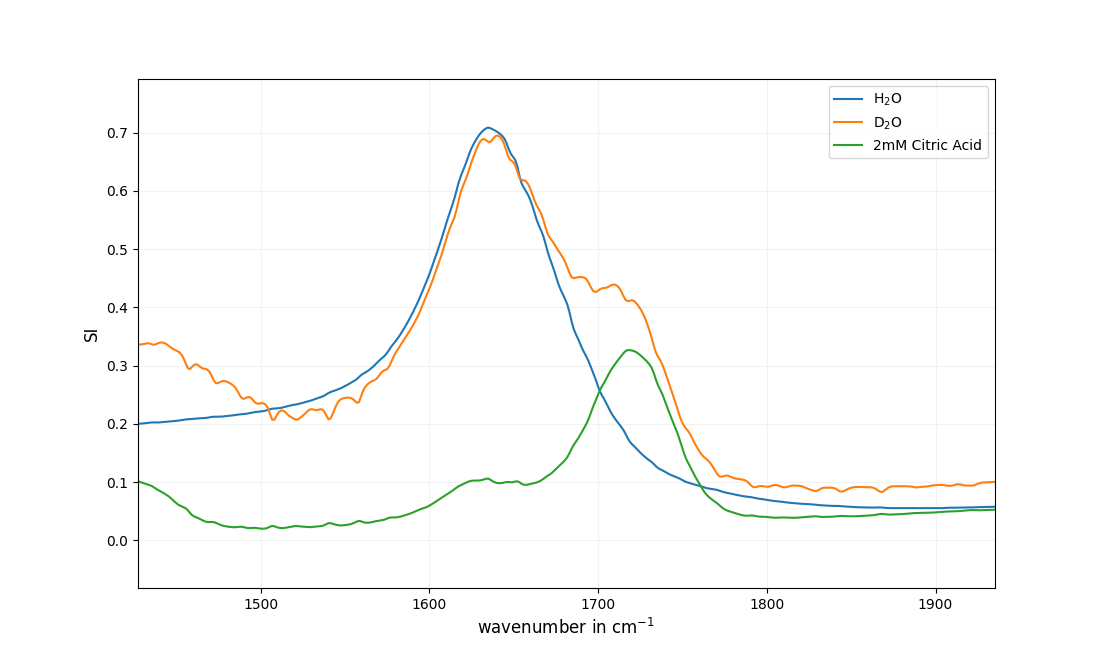
\includegraphics[scale=0.65]{water_citricacid_upclose.png}
			\caption{Infrarotspektrum von Wasser, Deuteriumoxid und 2mM Citronensäure in Wasser. Die Extrema in dem Bereich von Wasser und Deuteriumoxid überlappen mit dem Peak von Citronensäure.}
			\label{fig:water_citricacid}
		\end{figure}
		
		
		\begin{figure}[H]
			\centering
			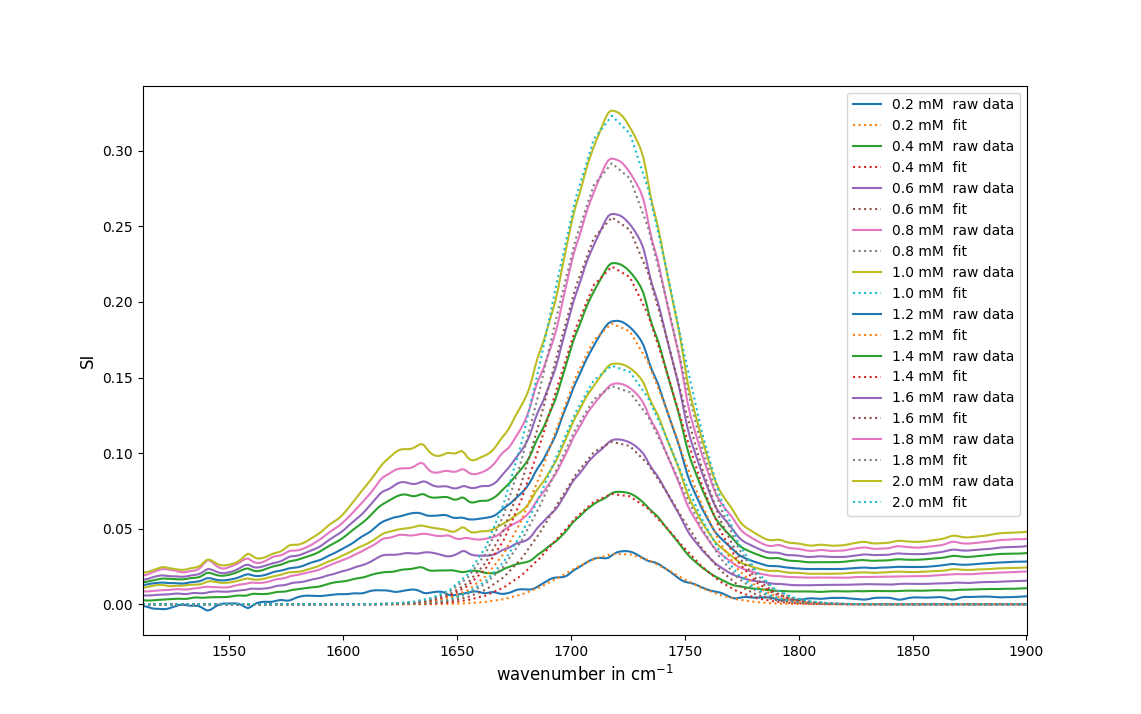
\includegraphics[scale=0.60]{Standardcurve_citricacid_fit.png}
			\caption{Infrarotspektrum der Verdünnungsreihe von Citronensäure in Wasser und der gaussche Fit des Maxima.}
			\label{fig:IR_Standardcurve}
		\end{figure}
	
	
	\addcontentsline{toc}{section}{References}
	\bibliographystyle{plainurl}
	\nocite{*}
	\bibliography{Literatur}
	\newpage
	
	
\end{document}